\documentclass[a4paper,oneside,12pt]{extreport}

\usepackage{mmap}
\usepackage[T2A]{fontenc}
\usepackage[utf8]{inputenc}
\usepackage[english,russian]{babel}


% Текст отчёта следует печатать, соблюдая следующие размеры полей:
% левое — 30 мм, правое — 15 мм, верхнее и нижнее — 20 мм.
\usepackage[left=20mm, right=15mm, top=15mm, bottom=15mm]{geometry}

% \setlength{\parindent}{1.25cm} % Абзацный отступ

\usepackage{setspace}
%\onehalfspacing % Полуторный интервал

\frenchspacing % Равномерные пробелы
\usepackage{indentfirst} % Красная строка

\usepackage{microtype}
\sloppy

\usepackage{titlesec}
\titlespacing*{\chapter}{0pt}{-30pt}{8pt}
\titlespacing*{\section}{\parindent}{*4}{*4}
\titlespacing*{\subsection}{\parindent}{*4}{*4}
\titleformat{\chapter}{\LARGE\bfseries}{\thechapter}{20pt}{\LARGE\bfseries}
\titleformat{\section}{\Large\bfseries}{\thesection}{40pt}{\Large\bfseries}

\usepackage{graphicx}
\usepackage{caption}

\usepackage[unicode,pdftex]{hyperref}
\hypersetup{hidelinks}

%% title begin
\usepackage{wrapfig}

\makeatletter
	\def\vhrulefill#1{\leavevmode\leaders\hrule\@height#1\hfill \kern\z@}
\makeatother
%% title end

%% begin code
\usepackage{listings}
\usepackage{xcolor}

\lstset{
	basicstyle=\footnotesize\ttfamily,
	breakatwhitespace=true,
	breaklines=true,
	commentstyle=\color{gray},
	frame=single,
	keywordstyle=\color{blue},
	stringstyle=\color{red},
	tabsize=8
}

\lstdefinestyle{lispinline}{
	frame=none,
	language=Lisp
}

\newcommand{\code}[1]{\texttt{#1}}
%% end code

%% begin theorem
\usepackage{amsthm}

\makeatletter
\newtheoremstyle{indented}
	{}% measure of space to leave above the theorem
	{}% measure of space to leave below the theorem
	{}% name of font to use in the body of the theorem
	{\parindent}% measure of space to indent
	{\bfseries}% name of head font
	{.}% punctuation between head and body
	{ }% space after theorem head; " " = normal interword space
	{}% header specification (empty for default)
\makeatother

\theoremstyle{indented}

\newtheorem{definition}{Определение}[section]
\newtheorem{example}{Пример}[section]
\newtheorem{theorem}{Теорема}[section]
\newtheorem{task}{Задание}

\makeatletter
\DeclareRobustCommand\bfseriesitshape{%
	\not@math@alphabet\itshapebfseries\relax
	\fontseries\bfdefault
	\fontshape\itdefault
	\selectfont
}
\makeatother

\DeclareTextFontCommand{\textbfit}{\bfseriesitshape}
\DeclareTextFontCommand{\define}{\bfseriesitshape}
%% end theorem

%% begin columns
\usepackage{etoolbox,refcount}
\usepackage{multicol}

\newcounter{countitems}
\newcounter{nextitemizecount}
\newcommand{\setupcountitems}{%
	\stepcounter{nextitemizecount}%
	\setcounter{countitems}{0}%
	\preto\item{\stepcounter{countitems}}%
}
\makeatletter
\newcommand{\computecountitems}{%
	\edef\@currentlabel{\number\c@countitems}%
	\label{countitems@\number\numexpr\value{nextitemizecount}-1\relax}%
}
\newcommand{\nextitemizecount}{%
	\getrefnumber{countitems@\number\c@nextitemizecount}%
}
\newcommand{\previtemizecount}{%
	\getrefnumber{countitems@\number\numexpr\value{nextitemizecount}-1\relax}%
}
\makeatother
\newenvironment{AutoMultiColItemize}{%
	\ifnumcomp{\nextitemizecount}{>}{3}{\begin{multicols}{2}}{}%
		\setupcountitems\begin{itemize}}%
		{\end{itemize}%
		\unskip\computecountitems\ifnumcomp{\previtemizecount}{>}{3}{\end{multicols}}{}}
\makeatother
\newenvironment{AutoMultiColEnumerate}{%
	\ifnumcomp{\nextitemizecount}{>}{3}{\begin{multicols}{2}}{}%
		\setupcountitems\begin{enumerate}}%
		{\end{enumerate}%
		\unskip\computecountitems\ifnumcomp{\previtemizecount}{>}{3}{\end{multicols}}{}}
%% end columns



\begin{document}

\begin{titlepage}
	\noindent\begin{minipage}{0.05\textwidth}
		
\includegraphics[scale=0.3]{inc/bmstu.png}
	\end{minipage}
	\hfill
	\begin{minipage}{0.85\textwidth}\raggedleft
		\begin{center}
			\fontsize{12pt}{0.3\baselineskip}\selectfont \textbf{Министерство науки и высшего образования Российской Федерации \\ Федеральное государственное бюджетное образовательное учреждение \\ высшего образования \\ <<Московский государственный технический университет \\ имени Н.Э. Баумана \\ (национальный исследовательский университет)>> \\ (МГТУ им. Н.Э. Баумана)}
		\end{center}
	\end{minipage}

	\begin{center}
		\fontsize{12pt}{0.1\baselineskip}\selectfont
		\noindent\makebox[\linewidth]{\rule{\textwidth}{4pt}} \makebox[\linewidth]{\rule{\textwidth}{1pt}}
	\end{center}

	\begin{flushleft}
		\fontsize{12pt}{0.8\baselineskip}\selectfont 
		
		ФАКУЛЬТЕТ \uline{<<\textbf{Информатика и системы управления}>> \hfill}

		КАФЕДРА \uline{\mbox{\hspace{4mm}} <<\textbf{Программное обеспечение ЭВМ и информационные технологии}>> \hfill}
	\end{flushleft}

	\vfill

	\begin{center}
		\fontsize{20pt}{\baselineskip}\selectfont

		\uline{\textbf{ОТЧЁТ ПО ПРОИЗВОДСТВЕННОЙ ПРАКТИКЕ}}
	\end{center}
	
	\vfill
	
	\begin{flushleft}
		\fontsize{12pt}{0.7\baselineskip}\selectfont

		Студент \uline{\mbox{\hspace{44mm}} Богаченко Артём Евгеньевич \hfill}
		
		Группа \uline{\mbox{\hspace{64mm}} ИУ7-65Б \hfill}
		
		Тип практики \uline{\mbox{\hspace{44mm}} Производственная \hfill}
		
		Название предприятия \uline{\mbox{\hspace{26mm}} ООО~<<Эррайвал РУС>> \hfill}
	\end{flushleft}	

	\vfill

	\begin{table}[h!]
		\fontsize{12pt}{0.7\baselineskip}\selectfont

		\begin{signstabular}[0.55]{p{7.25cm} >{\centering\arraybackslash}p{4cm} >{\centering\arraybackslash}p{4cm}}
		Студент & \uline{\mbox{\hspace*{4cm}}} & \uline{\hfill \textbf{Богаченко А. Е.} \hfill} \\
		& \scriptsize \textit{подпись, дата} & \scriptsize \textit{фамилия, и.о.}
		\end{signstabular}
	
		\vspace{\baselineskip}

		\begin{signstabular}[0.55]{p{7.25cm} >{\centering\arraybackslash}p{4cm} >{\centering\arraybackslash}p{4cm}}
			Руководитель практики & \uline{\mbox{\hspace*{4cm}}} & \uline{\hfill \textbf{Толпинская Н. Б.} \hfill} \\
			\mbox{\hspace*{1cm}} \scriptsize (от университета) & \scriptsize \textit{подпись, дата} & \scriptsize \textit{фамилия, и.о.}
		\end{signstabular}

		\vspace{\baselineskip}
		
		\begin{signstabular}[0.55]{p{7.25cm} >{\centering\arraybackslash}p{4cm} >{\centering\arraybackslash}p{4cm}}
			Руководитель практики & \uline{\mbox{\hspace*{4cm}}} & \uline{\hfill \textbf{Холодная Т. Ю.} \hfill} \\
			\mbox{\hspace*{1cm}} \scriptsize (от предприятия) & \scriptsize \textit{подпись, дата} & \scriptsize \textit{фамилия, и.о.}
		\end{signstabular}
	
		\vspace{\baselineskip}
		
		\begin{signstabular}[0.55]{p{7.25cm} >{\centering\arraybackslash}p{4cm} >{\centering\arraybackslash}p{4cm}}
			Оценка~~\uline{\hfill}
		\end{signstabular} 
	 
	\end{table}

	\vfill

	\begin{center}
		\normalsize \textit{\the\year~г.}
	\end{center}
\end{titlepage}

\section*{Практическая часть л.р.16}

\begin{task}
    Используя хвостовую рекурсию, разработать программу, позволяющую найти:

    \begin{enumerate}
        \item факториал числа;
        \item n-ое число Фибоначчи.
    \end{enumerate}

    \begin{lstlisting}[language=Prolog]
DOMAINS 
	number = integer

PREDICATES
	factorial(number, number, number).
	factorialWrapper(number, number).
	
CLAUSES
	factorial(0, Res, Res) :- !.
	factorial(Number, Current, Res) :- 
		NextNumber = Number - 1,
		Mult = Current * Number,
		factorial(NextNumber, Mult, Res).
	
	factorialWrapper(Number, -1) :- Number < 0, !. % Error. 
	factorialWrapper(Number, Res) :- factorial(Number, 1, Res).
	
GOAL
	% factorialWrapper(5, Result).
	% factorialWrapper(-5, Result).	
	factorialWrapper(0, Result).
\end{lstlisting}

    \newpage

    \begin{figure}[ht!]
    \centering{
        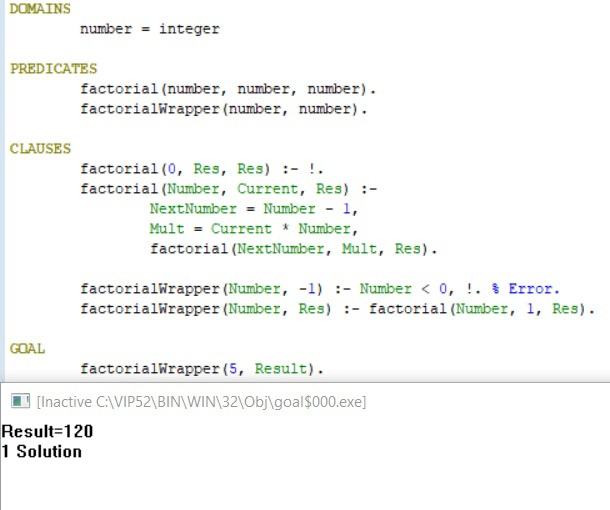
\includegraphics[width=0.9\textwidth]{img/res_lab_18/1.jpg}
        \caption{Факториал числа}}
    \end{figure}

    \begin{figure}[ht!]
        \centering{
            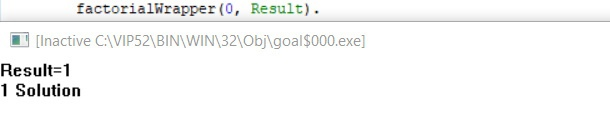
\includegraphics[width=0.9\textwidth]{img/res_lab_18/2.jpg}
            \caption{Факториал числа}}
    \end{figure}

    \begin{figure}[ht!]
    \centering{
        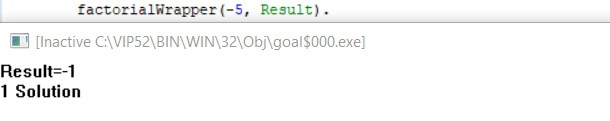
\includegraphics[width=0.9\textwidth]{img/res_lab_18/3.jpg}
        \caption{Факториал числа}}
    \end{figure}
    
    \begin{figure}[ht!]
        \centering{
            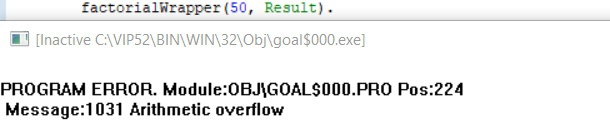
\includegraphics[width=0.9\textwidth]{img/res_lab_18/4.jpg}
            \caption{Факториал числа}}
    \end{figure}

    \newpage

    \begin{lstlisting}[language=Prolog]
DOMAINS 
	number = integer

PREDICATES
	fibonacci(number, number, number, number).
	fibonacciWrapper(number, number).

CLAUSES
	fibonacci(1, Prev, _, Prev) :- !.
	fibonacci(Number, Prev, Current, Res) :-
		NewNumber = Number - 1,
		Newprev = Current,
		NewCurrent = Prev + Current,
		fibonacci(NewNumber, NewPrev, NewCurrent, Res).
	
	
	fibonacciWrapper(Number, -1) :- Number < 1, !. % Error.
	fibonacciWrapper(Number, Res) :- fibonacci(Number, 1, 1, Res).
	
	
GOAL
	% fibonacciWrapper(-15, Result).
	% fibonacciWrapper(1, Result).
	% fibonacciWrapper(2, Result).
	% fibonacciWrapper(3, Result).
	fibonacciWrapper(8, Result).
    \end{lstlisting}

    \begin{figure}[ht!]
    \centering{
        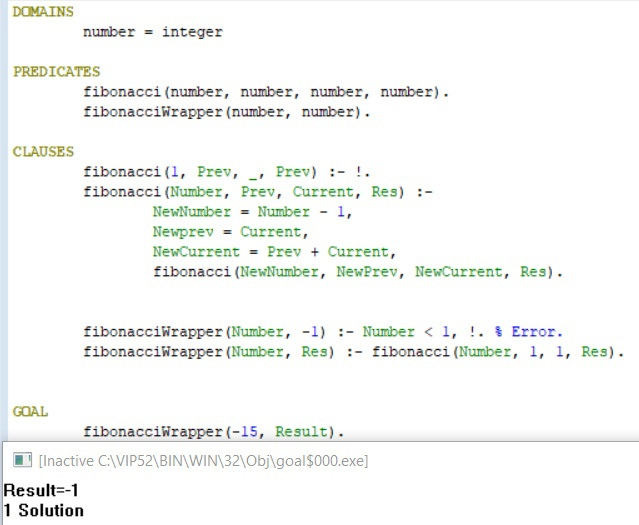
\includegraphics[width=0.9\textwidth]{img/res_lab_18/5.jpg}
        \caption{Фибоначчи}}
    \end{figure}
    
    \begin{figure}[ht!]
        \centering{
            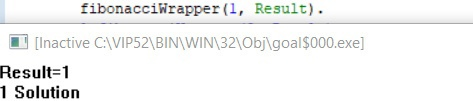
\includegraphics[width=0.9\textwidth]{img/res_lab_18/6.jpg}
            \caption{Фибоначчи}}
    \end{figure}

    \begin{figure}[ht!]
        \centering{
            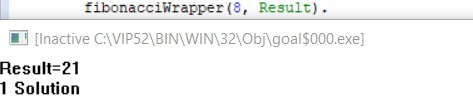
\includegraphics[width=0.9\textwidth]{img/res_lab_18/7.jpg}
            \caption{Фибоначчи}}
    \end{figure}

\end{task}

\newpage

\section*{Практическая часть л.р.17}

\begin{task}
    Используя хвостовую рекурсию, разработать эффективную программу, позволяющую:

    \begin{enumerate}
        \item найти длину списка (по верхнему уровню);
        \item найти сумму элементов числового списка;
        \item найти сумму элементов числового списка, стоящих на нечетных позициях
        исходного списка (нумерация от 0).
    \end{enumerate}

    Убедиться в правильности результатов.

    Длина списка.
    \begin{lstlisting}[language=Prolog]
DOMAINS
    list = integer*.

PREDICATES
    length(list, integer, integer).
    lengthWapper(list, integer).
    
CLAUSES
    length([], Res, Res) :- !.
    length([_|T], CurrValue, Res) :- 
        NewCurrValue = CurrValue + 1,
        length(T, NewCurrValue, Res). 
    
    lengthWapper(L, Res) :- length(L, 0, Res).

GOAL
    % lengthWapper([1, 2, 3], Result).
    % lengthWapper([], Result).
    lengthWapper([1, 2, 3, 1, 2, 3, 1, 2, 3], Result).
    \end{lstlisting}

    Сумма элементов числового списка.
    \begin{lstlisting}[language=Prolog]
DOMAINS
    list = integer*.

PREDICATES
    sum(list, integer, integer).
    sumWapper(list, integer).
    
CLAUSES
    sum([], Res, Res) :- !.
    sum([H|T], CurrValue, Res) :- 
        NewCurrValue = CurrValue + H,
        sum(T, NewCurrValue, Res). 
    
    sumWapper(L, Res) :- sum(L, 0, Res).

GOAL
    % sumWapper([1, 2, 3], Result).
    % sumWapper([], Result).
    sumWapper([1, 2, 3, 1, 2, 3, 1, 2, 3], Result).
    \end{lstlisting}

    \newpage
    
    Сумма элементов числового списка, стоящих на нечетных позициях.
    \begin{lstlisting}[language=Prolog]
DOMAINS
    list = integer*.
    flag = integer. 

PREDICATES
    sum_odd(list, integer, integer, flag).
    sum_oddWapper(list, integer).
    
CLAUSES
    sum_odd([], Res, Res, _) :- !.
    sum_odd([_|T], CurrValue, Res, 0) :- sum_odd(T, CurrValue, Res, 1).
    
    sum_odd([H|T], CurrValue, Res, 1) :- 
        NewCurrValue = CurrValue + H,
        sum_odd(T, NewCurrValue, Res, 0).
    
    sum_oddWapper(L, Res) :- sum_odd(L, 0, Res, 0). 

GOAL
    % sum_oddWapper([1, 2, 3], Result).
    %sum_oddWapper([], Result).
    %sum_oddWapper([1, 2, 3, 1, 2, 3, 1, 2, 3], Result).
    sum_oddWapper([1, 2, 3, 4, 5], Result).
    %sum_oddWapper([1], Result).
    \end{lstlisting}

    \begin{figure}[ht!]
    \centering{
        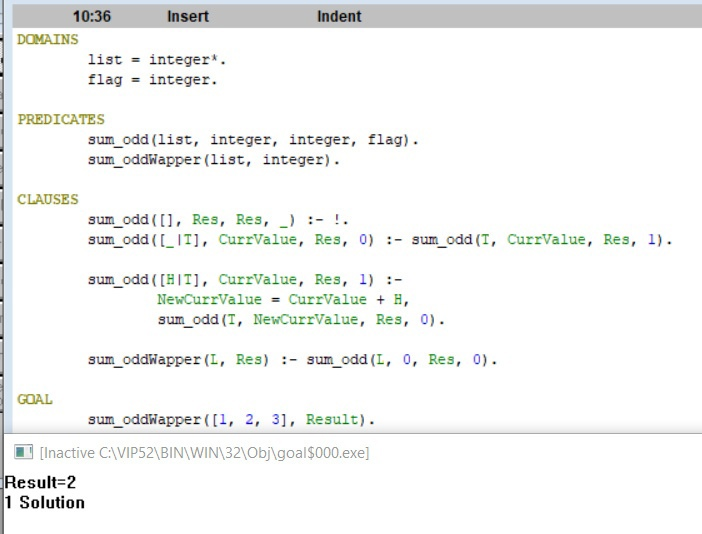
\includegraphics[width=0.9\textwidth]{img/res_lab_19/1.jpg}
        \caption{Сумма элементов числового списка, стоящих на нечетных позициях.}}
    \end{figure}
    
    \begin{figure}[ht!]
        \centering{
            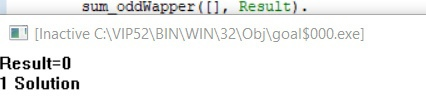
\includegraphics[width=0.9\textwidth]{img/res_lab_19/2.jpg}
            \caption{Сумма элементов числового списка, стоящих на нечетных позициях.}}
    \end{figure}

    \begin{figure}[ht!]
        \centering{
            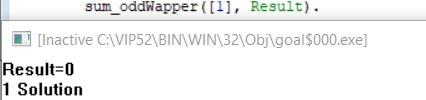
\includegraphics[width=0.9\textwidth]{img/res_lab_19/3.jpg}
            \caption{Сумма элементов числового списка, стоящих на нечетных позициях.}}
    \end{figure}
\end{task}

\newpage


\end{document}